% Template:     Informe LaTeX
% Documento:    Archivo principal
% Versión:      8.2.7 (21/08/2023)
% Codificación: UTF-8
%
% Autor: Pablo Pizarro R.
%        pablo@ppizarror.com
%
% Manual template: [https://latex.ppizarror.com/informe]
% Licencia MIT:    [https://opensource.org/licenses/MIT]

% CREACIÓN DEL DOCUMENTO
\documentclass[
	spanish, % Idioma: spanish, english, etc.
	letterpaper, oneside
]{article}

\usepackage{multirow}
\usepackage{caption}



% INFORMACIÓN DEL DOCUMENTO
\def\documenttitle {Tarea 1 Data Science for Social Network Analysis}
\def\documentsubtitle {}
\def\documentsubject {}

\def\documentauthor {Bryan Cabezas}
\def\coursename {}
\def\coursecode {IN7600}

\def\universityname {Universidad de Chile}
\def\universityfaculty {Facultad de Ciencias Físicas y Matemáticas}
\def\universitydepartment {Departamento de Ingeniería Industrial}
\def\universitydepartmentimage {departamentos/dii}
\def\universitydepartmentimagecfg {height=1.57cm}
\def\universitylocation {Santiago de Chile}

% INTEGRANTES, PROFESORES Y FECHAS
\def\authortable {
	\begin{tabular}{ll}
		Integrantes:
		& \begin{tabular}[t]{l}
			Bryan Cabezas Sandoval\\
		\end{tabular} \\
		Profesor:
		& \begin{tabular}[t]{l}
            Richard Weber
		\end{tabular} \\
		Auxiliar:
		& \begin{tabular}[t]{l}
			Dimitri Loaiza \\
            Susana Rojas
		\end{tabular} \\
		Ayudantes:
		& \begin{tabular}[t]{l}
			Víctor Bunster
		\end{tabular} \\
		& \\
		\multicolumn{2}{l}{Fecha de entrega: 01 de Abril del 2026} \\
		\multicolumn{2}{l}{\universitylocation}
	\end{tabular}
}

% IMPORTACIÓN DEL TEMPLATE
\input{template}
%\usepackage[a4paper,margin=2.5cm]{geometry}
% INICIO DE PÁGINAS
\begin{document}
% PORTADA
\templatePortrait

% CONFIGURACIÓN DE PÁGINA Y ENCABEZADOS
\templatePagecfg

% --- AQUÍ AGREGAS EL ÍNDICE ---
\newpage % Opcional: para que el índice empiece en una página nueva
\tableofcontents
\newpage % Opcional: para que tu contenido empiece después del índice
% ------------------------------


% CONFIGURACIONES FINALES
\templateFinalcfg
% ======================= INICIO DEL DOCUMENTO =======================

\section{Carga de datos y manejo básico de Gephi}
Para la creación de la red, se utilizó la base de datos de Spotify. El dataset df\_edges.csv contiene las colaboraciones entre artistas, mientras que el dataset df\_nodes.csv contiene la información individual de cada artista, como su popularidad, seguidores y géneros musicales. Las colaboraciones entre artistas se utilizarón para crear las aristas de la red, mientras que la información individual de cada artista se utilizó para asignar atributos a los nodos. De manera que los nodos representan a los artistas y las aristas representan las colaboraciones entre ellos.

El artista escogido para el análisis es: 'Polimá Westcoast' con nivel 2, donde presenta 884 nodos totales y 8591 artistas.

Para la visualización se utilizó el algoritmo Force Atlas con una repulsión de 20000. La imagen de la social network se muestra a continuación:
\begin{figure}[ht!]
    \centering
    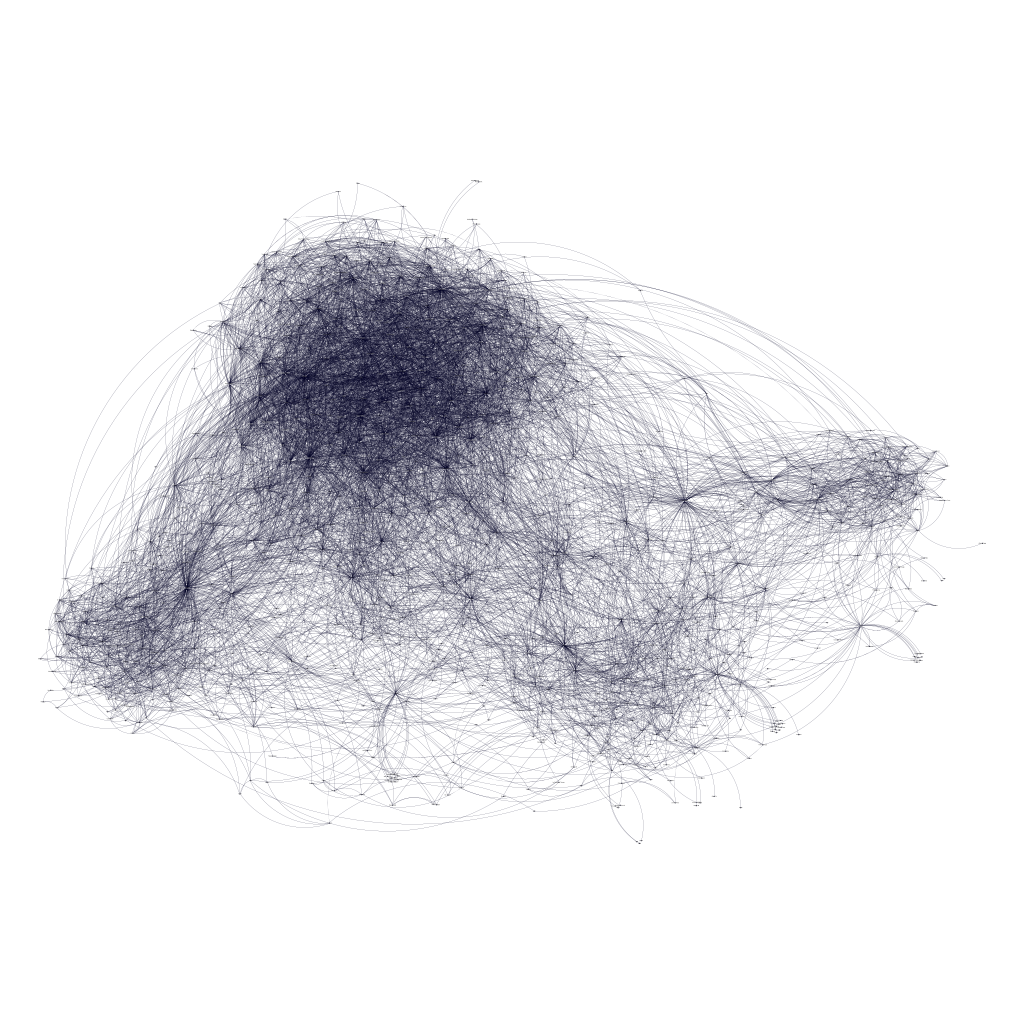
\includegraphics[width=0.5\textwidth]{PolimaWestcolNetwork.png}
    \caption{Social Network de Polimá Westcoast}
    \label{fig:PolimáWestcoastSocialNetwork}
\end{figure}




\section{Pregunta 2.1}
Sí, existe una relación clara entre las distintas medidas de centralidad para los nodos principales de la red, como se observa en la figuras \ref{fig:Degree2.1}, \ref{fig:betweenness2.1}, \ref{fig:Closeness2.1} y \ref{fig:PageRank2.1}. Generalmente, un artista con un alto degree (muchas colaboraciones) termina funcionando como una "puerta de entrada" para nuevos talentos, lo que eleva su betweenness al conectar a esos artistas emergentes con el resto de la industria. Al estar tan bien conectado, este artista también reduce la distancia promedio hacia los demás nodos, logrando un closeness alto, lo que significa que cualquier tendencia que pase por él llega a toda la comunidad en muy pocos pasos. Asi tambien, al colaborar con artistas de alto prestigio, su influeza se amplifica, lo que se refleja en un PageRank elevado. Esto mismo se puede observar en las figuras \ref{fig:DegreeBetweenness2.1} y \ref{fig:PageRankCloseness2.1}, donde se muestra la relación entre estas medidas, confirmando que los artistas con mayor cantidad de colaboraciones (degree) también tienden a ser los puentes más importantes (betweenness), y aquellos con mayor influencia (PageRank) suelen estar más cerca de toda la red (closeness).

Esto se ve claramente en el género urbano con artistas como J Balvin. Su alto degree es consecuencia directa de la cultura del reggaetón, donde los 'remixes' y colaboraciones constantes son la norma. Ese mismo volumen de trabajo le da un betweenness elevado, ya que actúa como el puente que conecta nichos locales (artistas que apenas están empezando) con el mercado global. Asimismo, su alto closeness confirma su capacidad de influencia, al estar posicionado en el centro estratégico de la red, demostrando que tiene el poder de viralizar estilos o canciones de manera mucho más eficiente que un artista periférico. Finalmente, su PageRank elevado demuestra que el artista no solo es popular por sí mismo, sino que colabora con otros artistas de alto prestigio. 

\begin{figure}[ht!]
    \centering
    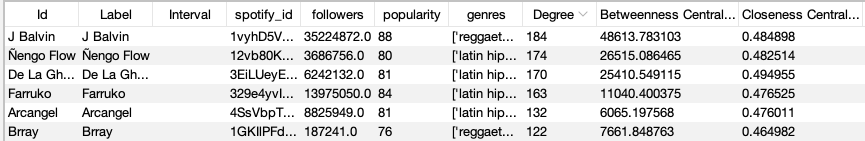
\includegraphics[width=0.7\textwidth]{Alto Degree 2.1.png}
    \caption{Artistas con mayor medida Degree}
    \label{fig:Degree2.1}
\end{figure}

\begin{figure}[ht!]
    \centering
    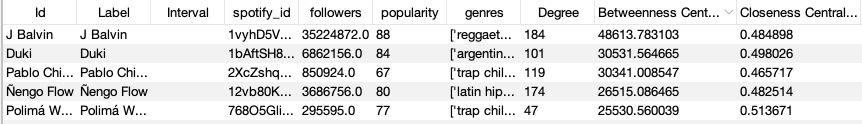
\includegraphics[width=0.7\textwidth]{Alto betweenness 2.1.png}
    \caption{Artistas con mayor medida Betweenness}
    \label{fig:betweenness2.1}
\end{figure}

\begin{figure}[ht!]
    \centering
    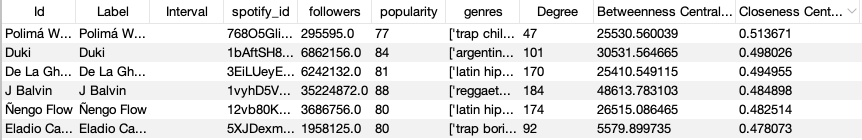
\includegraphics[width=0.7\textwidth]{Alto clossnes 2.1.png}
    \caption{Artistas con mayor medida Closeness}
    \label{fig:Closeness2.1}
\end{figure}

\begin{figure}[ht!]
    \centering
    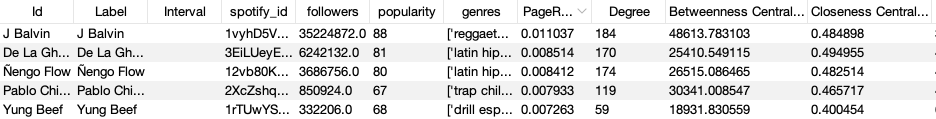
\includegraphics[width=0.7\textwidth]{Alto PageRank.png}
    \caption{Artistas con mayor medida PageRank}
    \label{fig:PageRank2.1}
\end{figure}

%\begin{figure}[ht!]
%    \centering
%    \includegraphics[width=0.7\textwidth]%{RelacionDegreeTamañoConBetweennessColor.png}
%    \caption{Relación de Degree (tamaño) y Betweenness (color)}
%    \label{fig:DegreeBetweenness2.1}
%\end{figure}

%\begin{figure}[ht!]
%    \centering
%    \includegraphics[width=0.7\textwidth]%{RelacionPageRankTamañoConClossennessColor.png}
%    \caption{Relación de PageRank (tamaño) y Closeness (color)}
%    \label{fig:PageRankCloseness2.1}
%\end{figure}

\vspace{0.5em} % Espacio estético arriba
\begin{center}
    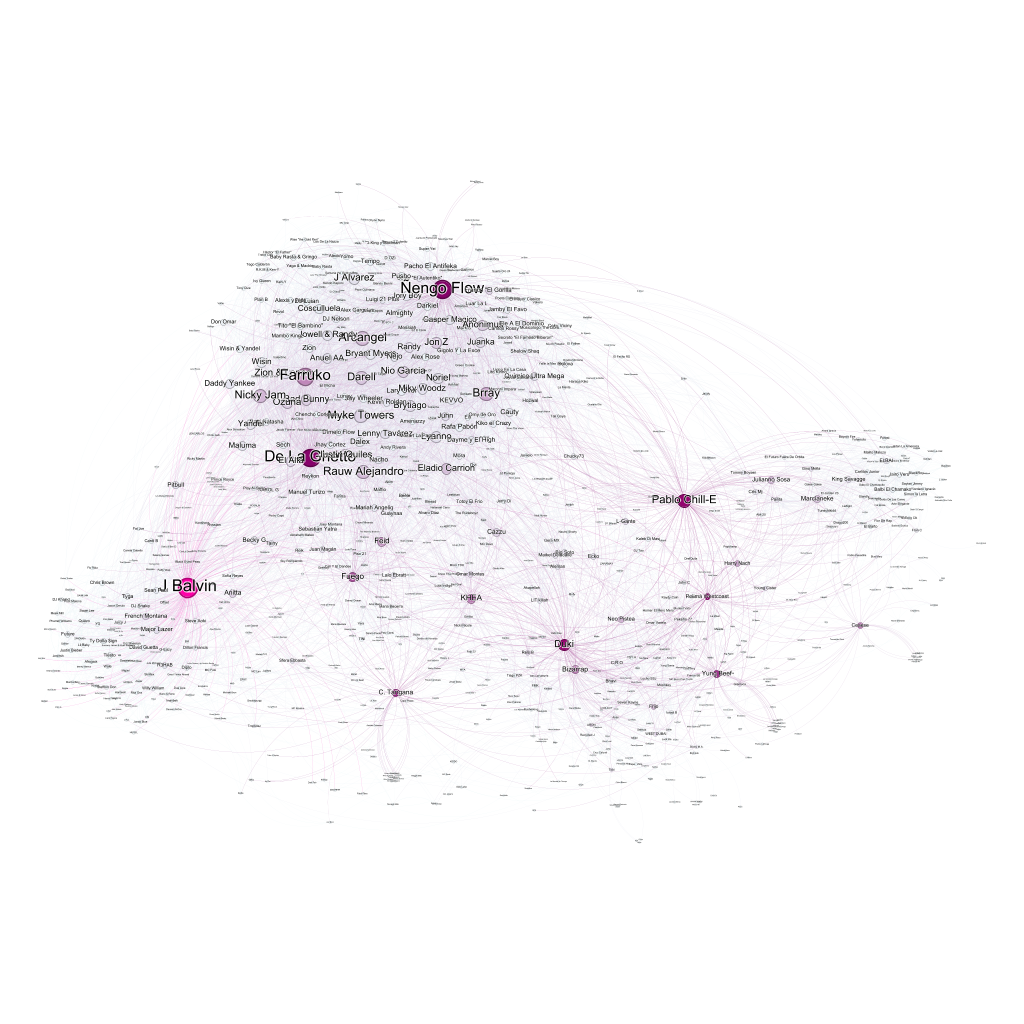
\includegraphics[width=0.6\textwidth]{RelacionDegreeTamañoConBetweennessColor.png} 
    \captionof{figure}{Relación de Degree (tamaño) y Betweenness (color)}
    \label{fig:DegreeBetweenness2.1}
\end{center}
\vspace{0.5em} % Espacio estético abajo

\vspace{0.5em} % Espacio estético arriba
\begin{center}
    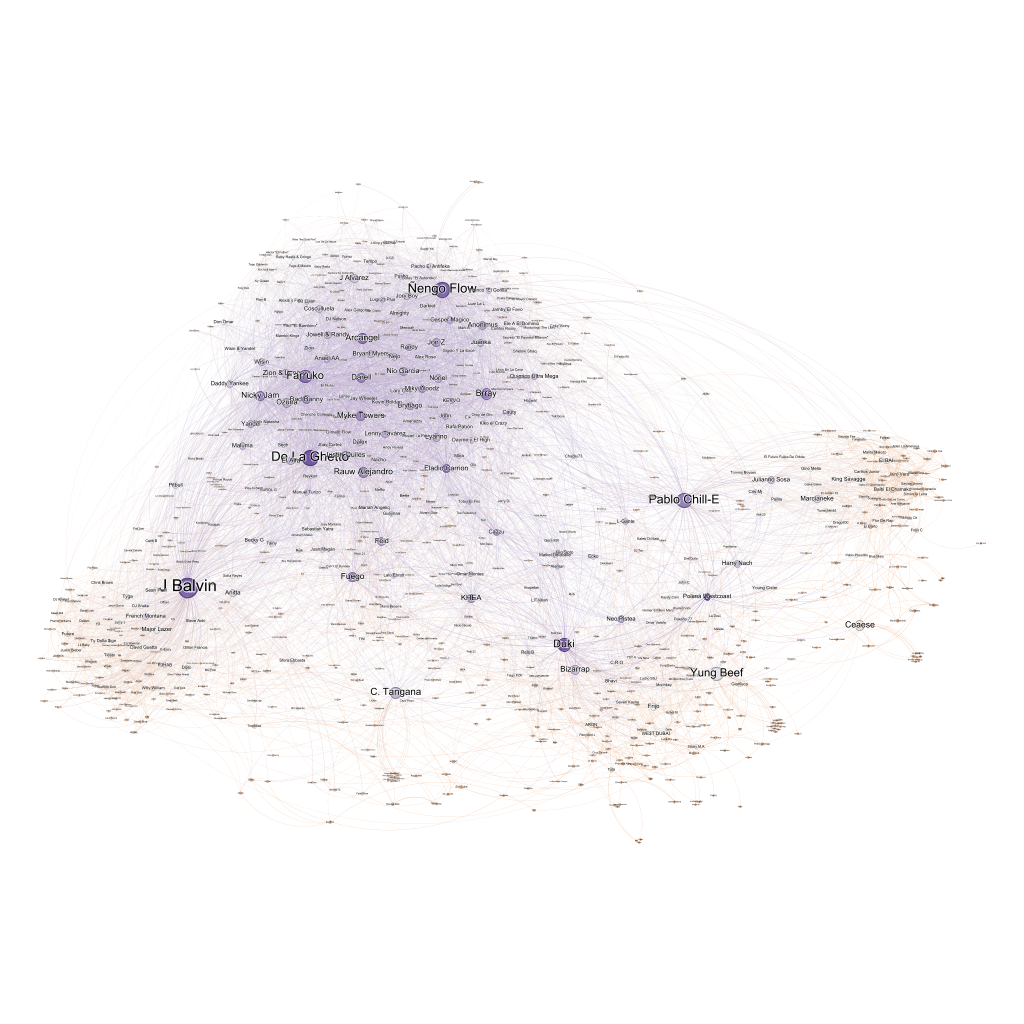
\includegraphics[width=0.6\textwidth]{RelacionPageRankTamañoConClossennessColor.png} 
    \captionof{figure}{Relación de PageRank (tamaño) y Closeness (color)}
    \label{fig:PageRankCloseness2.1}
\end{center}
\vspace{1em} % Espacio estético abajo




\section{Pregunta 2.2}
Cuando se realiza la asignación de color mediante la popularidad y el tamaño según el Degree, se observa que no siempre existe una relación lineal, ya que hay artistas extremadamente populares cuyas canciones propias son suficientes para mantener su estatus sin necesidad de colaborar constantemente. Esto ocurre por ejemplo con Bad Bunny de la figura \ref{fig:ArtistasPorPopularidad2.2} , quien posee la popularidad máxima de 100, pero un degree de 95, lejos del máximo de la red de 184. Esto indica que, aunque los artistas con mayor conectividad suelen ser bien famosos, existen superestrellas que no dependen de un alto volumen de vínculos (colaboraciones) para liderar el ranking de popularidad, como el ejemplo mencionado. Además, si se representa los nodos según su Degree, donde más grande es el nodo, más colaboraciones tiene, y más rosado el color significa mayor popularidad, se observa nuevamente el patron con el artista en la figura \ref{fig:SocialNetworkBadBunny2.2}.


\begin{figure}[ht!]
    \centering
    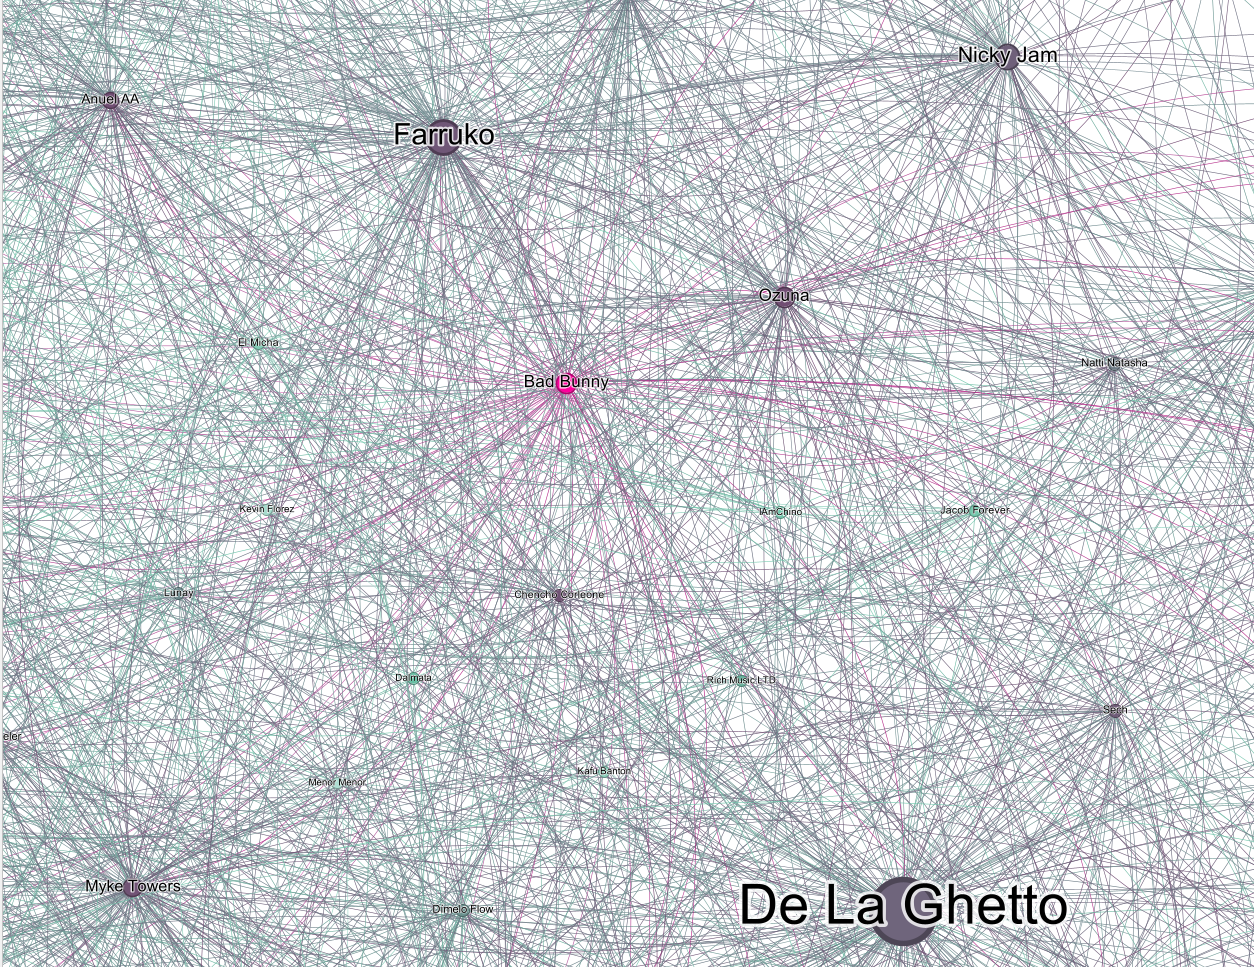
\includegraphics[width=0.7\textwidth]{BadBunnyPopularityBetweennessNetwork2.2.png}
    \caption{Social Network con color de popularidad y tamaño según Degree del artista Bad Bunny}
    \label{fig:SocialNetworkBadBunny2.2}
\end{figure}

\begin{figure}[ht!]
    \centering
    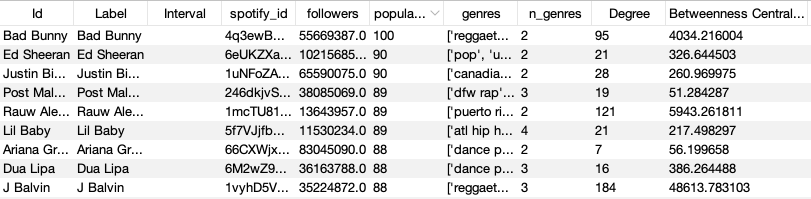
\includegraphics[width=0.7\textwidth]{BadBunnyPopularityBetweenness2.2.png}
    \caption{Artistas ordenados por mayor popularidad}
    \label{fig:ArtistasPorPopularidad2.2}
\end{figure}

Por otro lado, al analizar el color por seguidores y el tamaño del nodo por Betweenness, el patrón cambia según el género musical como se muestra en las figuras \ref{fig:SocialNetworkEdSheeran2.2} y \ref{fig:ArtistasPorFollowers2.2}. Artista de pop global como Ed Sheeran lideran en cantidad de seguidores pero presenta un betweenness bajo. Esto se repite con los primeros 4 artistas del mismo género, lo cual sugiere que los artistas de pop tienden a colaborar dentro del mismo círculo consolidado, sin actuar como puentes hacia otros nichos. En contraste, artistas como Bad Bunny (quinto lugar) y J Balvin rompen este patrón, al presentar un Betweenness mucho más alto y con alto número de seguidores también. Esto demuestra que el género urbano tiene una mayor tendencia a la exploración de nuevos nichos, y a servir de puente para artistas emergentes,  generando una red mucho más integrada que la del pop.

\begin{figure}[ht!]
    \centering
    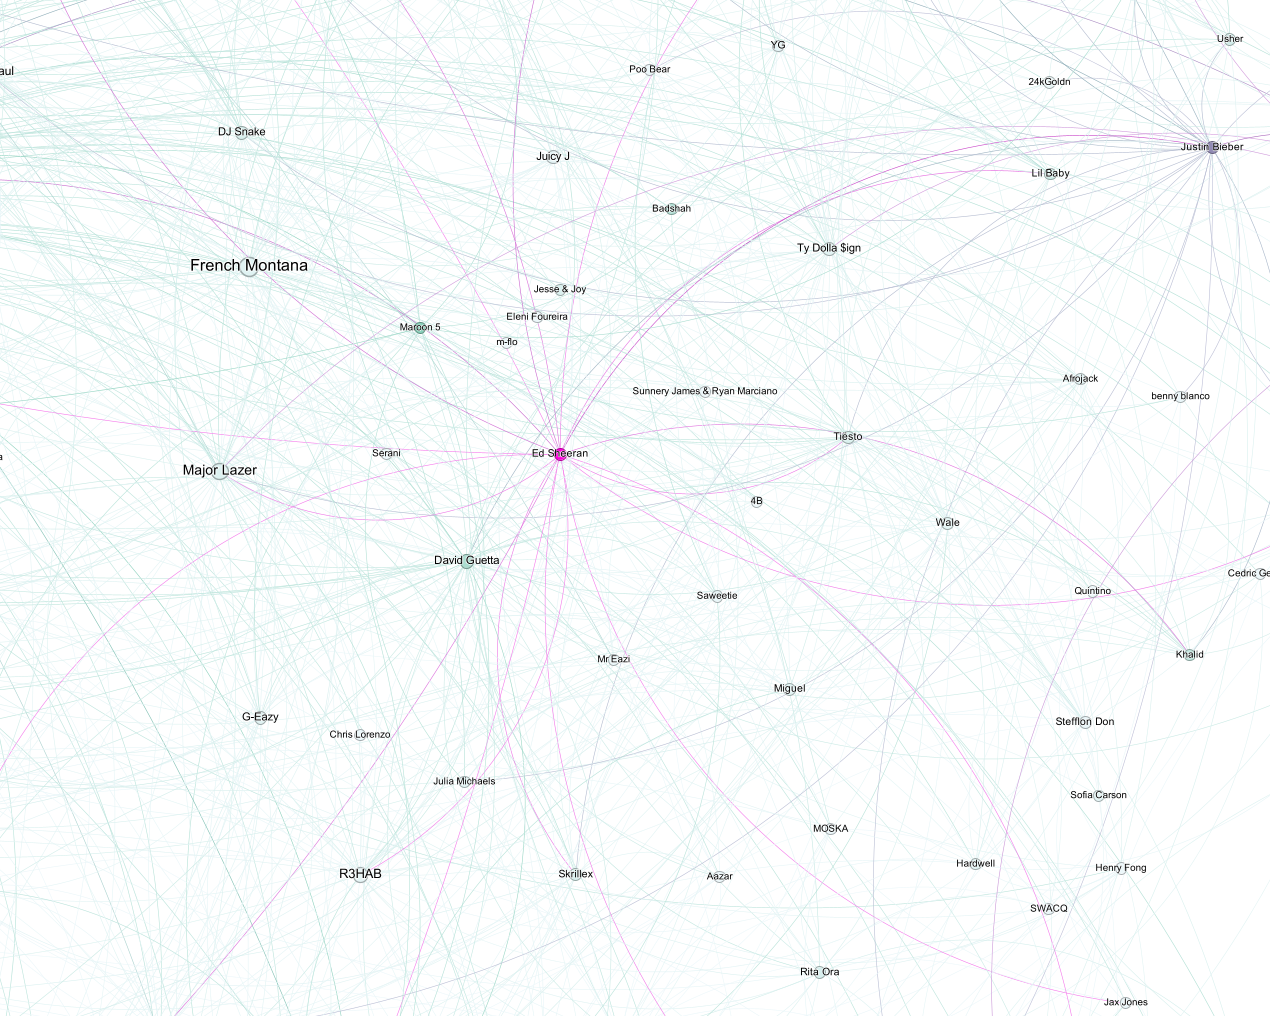
\includegraphics[width=0.7\textwidth]{EdSheeranFollowersNetwork2.2.png}
    \caption{Social Network con color de seguidores y tamaño según Betweenness del artista Ed Sheeran}
    \label{fig:SocialNetworkEdSheeran2.2}
\end{figure}

\begin{figure}[ht!]
    \centering
    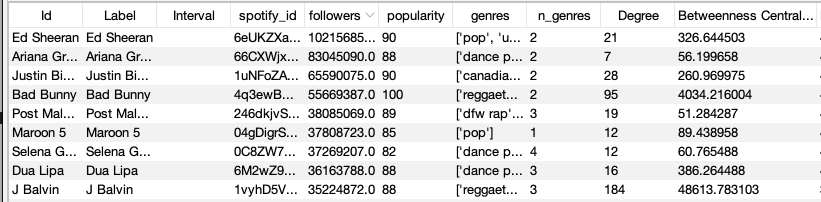
\includegraphics[width=0.7\textwidth]{FollowersOrdenados2.2.png}
    \caption{Artistas ordenados por mayor cantidad de seguidores}
    \label{fig:ArtistasPorFollowers2.2}
\end{figure}


\section{Pregunta 2.3}

\begin{tabular}{|l|l|}
\hline
Indicador & Valor \\
\hline
Grado medio & 19.437 \\
Diámetro & 4 \\
Radio & 2 \\
Largo medio de caminos mínimos & 2.869 \\
\hline
\end{tabular}


El indicador de grado medio de la red refuerzan que el género urbano presenta una comunidad hiperconectada, ya que indica que en promedio cada artista ha colaborado casi con 20 personas diferentes dentro de la misma red. Un diámetro de 4 significa que, en el peor de los casos (artistas muy alejados) se necesitan cuatro saltos para conectar dos artistas, y esto sumado a un radio de dos, confirma que es una red compacta. Finalmente un largo medio de caminos mínimos de 2.869, demuestra que en promedio cualquier par de artistas en la red están separados por menos de 3 colaboradores. Esto explica por qué el reggaetón se globaliza tan rápido, ya que la distancia social entre los artistas es mínima, lo que permite que las tendencias musicales se expandan con gran velocidad.




\section{Pregunta 2.4}
La medida de centralidad Degree representa a la cantidad de colaboraciones que ha realizado dicho artista. Un valor de Degree alto, significa que el artista ha colaborado de manera activa con múltiples otros artistas, mientras que un valor bajo refleja un artista con poca cantidad de colaboración variadas, quizás por más hermetismo o selectividad. Por otro lado, la medida Betweenness mide la capacidad de un nodo para actuar como puente entre distintas comunidades del grafo, es decir, un artista que conecta entremedio de vínculos. Un alto Betweenness sugiere que el artista puede conectar dos géneros musicales o nichos que de otro modo estarían aislados (como unir trap con el mercado global), y a la vez abrir puertas a talentos emergentes. Un bajo Betweenness, implica que el artista se mantiene dentro de su propio género sin expandir los vínculos de la red.

Al combinar ambas medidas, si un nodo posee alto degree y alto betweenness implica que es un artista con alta cantidad de colaboraciones y a la vez presenta una alta habilidad para adaptarse a distintos géneros musicales y generar puentes entre ellos; Un bajo degree y bajo betweenness significa que realiza pocas colaboraciones y se aisla en un genero; Un alto degree y bajo betweenness demuestra que es un artista con alta cantidad de colaboraciones, pero siempre dentro del mismo círculo cerrado; Un bajo degree y alto betweenness, también es posible, pero con artistas de culto, que aunque realizan pocas colaboraciones, estas son los únicos vínculos existentes entre géneros musicales distintos, entregando un rol de intermediación.



\section{Pregunta 2.5}

\begin{tabular}{|l|l|}
\hline
Indicador & Valor \\
\hline
Arista & Polimá Westcoast \\
Grado & 47 \\
Excentricidad & 2.0 \\
Closeness Centrality & 0.5147 \\
Betweenness Centrality & 25530 \\
Eigenvector Centrality & 0.1413 \\
\hline
\end{tabular}

Basado en los indicadores obtenidos, la relación de Polimá Westcoast con la industria musical se define como la de un conector de alto impacto. Con un Grado (Degree) de 47, el artista demuestra una actividad colaborativa muy superior al promedio(de 19.437), lo que valida la hipótesis de que es un artista activo y diversificado. Además, el valor de Betweeness Centrality de 25530 es alto, lo que confirma que Polimá no solo colabora mucho, sino que sus vínculos actúan como puentes para conectar artistas de generos variados (como bizarrap) con géneros adyacentes, lo que lo hace un nodo fundamental para la cohesión del grafo. Una Excentricidad de 2.0, demuestra que el artista está a una distancia máxima de solo dos saltos de cualquier otro miembro relevante de su red, lo cual tiene sentido al ser un artista con alto grado y betweenness, posicionandolo en un nodo que pueda propagar tendencias. Esto tambien se traduce a un Closeness Centrality de 0.5147, que indica que es un artista que solo necesita poco más de la mitad de los pasos para que toda la red sepa de cualquier tendencia, género o innovación musical que él adopte, al presentar una distancia promedio para llegar a cualquier otro artista muy corta (2.869). Finalmente, el Eigenvector Centrality de 0.1413, entrega una métrica relevente, ya que no solo cuenta sus conexiones, sino la importancia de estas. Este valor indica que Polimá no solo colabora con varios artistas, sino que lo hace con los más importantes, es decir con nodos con alto grado, consolidando un estatus de un artista con gran influenza y prestigio dentro del género urbano.

\section{Pregunta 2.6}

Al aplicar el algoritmo de detección de comunidades basado en modularidad, se identificaron 5 comunidades principales dentro de la red de Polimá Westcoast como se muestra en la figura \ref{fig:PolimaModularity2.6}. Al analizar la estructura, se observa que la mayoría se agrupan por país de origen / proximidad geográfica, lo que sugiere que las colaboraciones tienden a ser más frecuentes entre artistas del mismo país. Por ejemplo, la comunidad naranja está compuesta principalmente por Chilenos (DrefQuila, Pablo Chill-E, etc), la comunidad morada por Argentinos (donde se incluyen artistas como Villano Antillano, que no es de Argentina, pero se hizo conocido debido a su fuerte vínculo estructural de colaboración con Bizarrap), la comunidad rosada por artistas de República Dominicana. Sin embargo, este patrón geográfico se rompe en las comunidades con mayor jerarquía global de colaboraciones. La comunidad azul no es estrictamente nacional, al representar una fusión de mercados masivos donde artistas potentes de Colombia como J Balvin o Maluma se entrelazan con figuras del pop anglo y EMD (como Dua Lipa, Maroon 5, etc.), al realizar colaboraciones, evidenciando como el Reggaetón internacional actua como puente transnacional que conecta artistas de distintos países y géneros. Finalmente, la comunidad amarilla se define por una afinidad de género (Latin pop), donde artistas como Lele Pons o OneRepublic aparecen debido a sus colaboraciones estratégicas con nodos centrales de esta comunidad (como Sebastian Yatra), lo que demuestra que en la industria musical moderna, las colaboraciones pesan más que la nacionalidad de origen. Por otro lado, estos fenómenos de colaboración se confirman al analizar la métrica de Betweenness, donde los nodos más relevantes de cada comunidad no son necesariamente los que más colaboraciones realizan, sino aquellos que actuan como puentes criticos hacia otros grupos (comunidades). Por ejemplo, Polimá Westcoast o Pablo Chill-E, presentan Betweenness altos, al posicionarse como conectores fundamentales entre la escena chilena y el mercado latinoamericano como con Argentina, que ha hecho colaboraciones con Duki y Bizarrap o Puerto Rico, con Bad Bunny y Ñengo Flow. Esto permite abrir puertas a otros artistas de su comunidad para repetir ese patrón de colaboración internacional. Un caso similar ocurre con C. Tangana, quien ha colaborado con artistas de Colombia y Argentina, lo que lo posiciona como puente de artistas españoles hacia el mercado latinoamericano, y a su vez, artistas de otros países hacia el mercado español. Esto demuestra que el genero urbano tiene mayor tendencia a la exploración de nuevos nichos, y a servir de puente para artistas emergentes, creando una red más integrada. Adicionalmente, se observa que la comunidad verde presenta un valor de degree más alto que el resto, en los primeros artistas de esta comunidad, con una distribución muy similar. La comunidad naranja presenta un betweenness más homogeneo que las demás comunidades, presentando una disminución más gradual, sugiriendo una estructura más integrada. Por otro lado, la comunidad rosada presenta un valor de Degree más imparejo entre los artistas que lo componen, con artistas con un Degree muy alto (como el Alfa) y otros con un Degree muy bajo, lo que sugiere una estructura más jerárquica. 

%\vspace{0.5em} % Espacio estético arriba
\begin{center}
    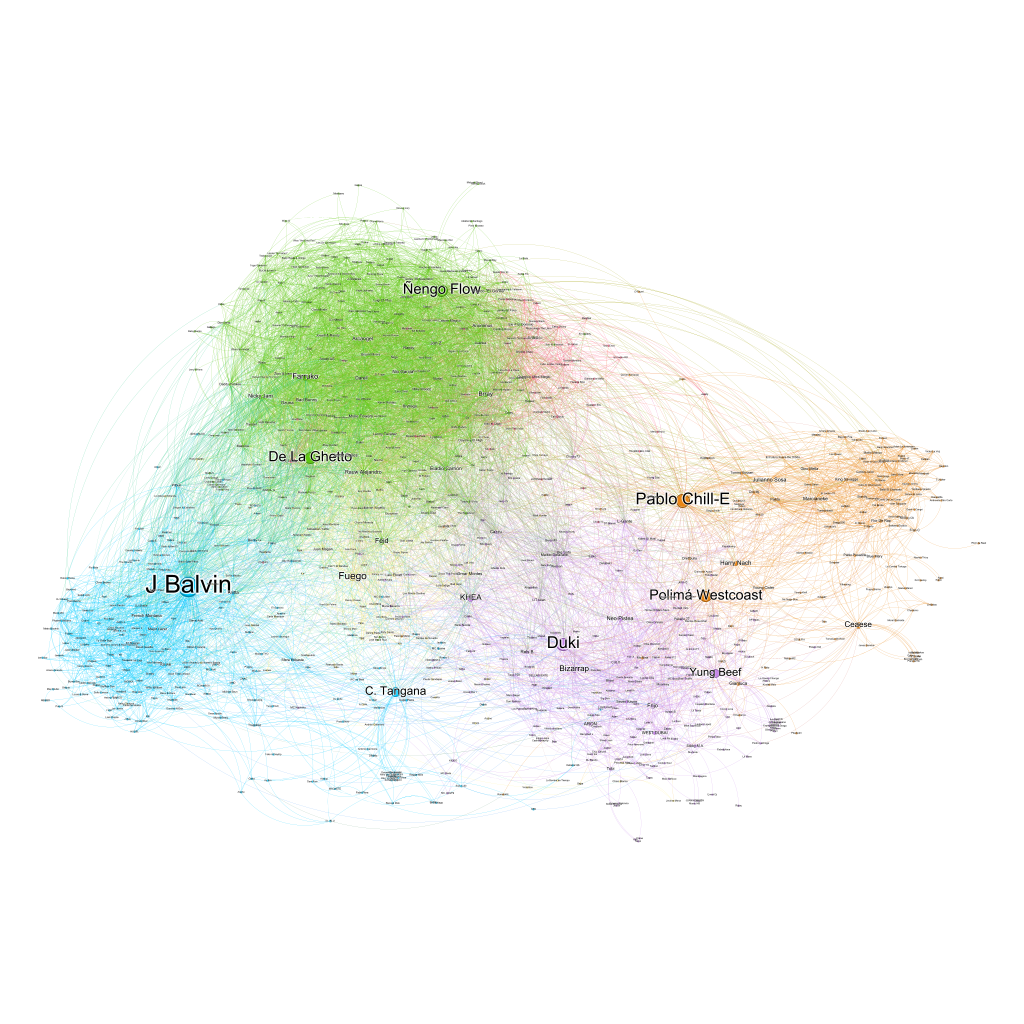
\includegraphics[width=1\textwidth]{PolimaWestcolModularity.png} 
    \captionof{figure}{Social Network de Polimá Westcoast con comunidades detectadas por modularidad y tamaño de nodo según Betweenness}
    \label{fig:PolimaModularity2.6}
\end{center}
%\vspace{-15em}
%\vspace{1em} % Espacio estético abajo

%\begin{figure}[ht!]
%    \centering
%    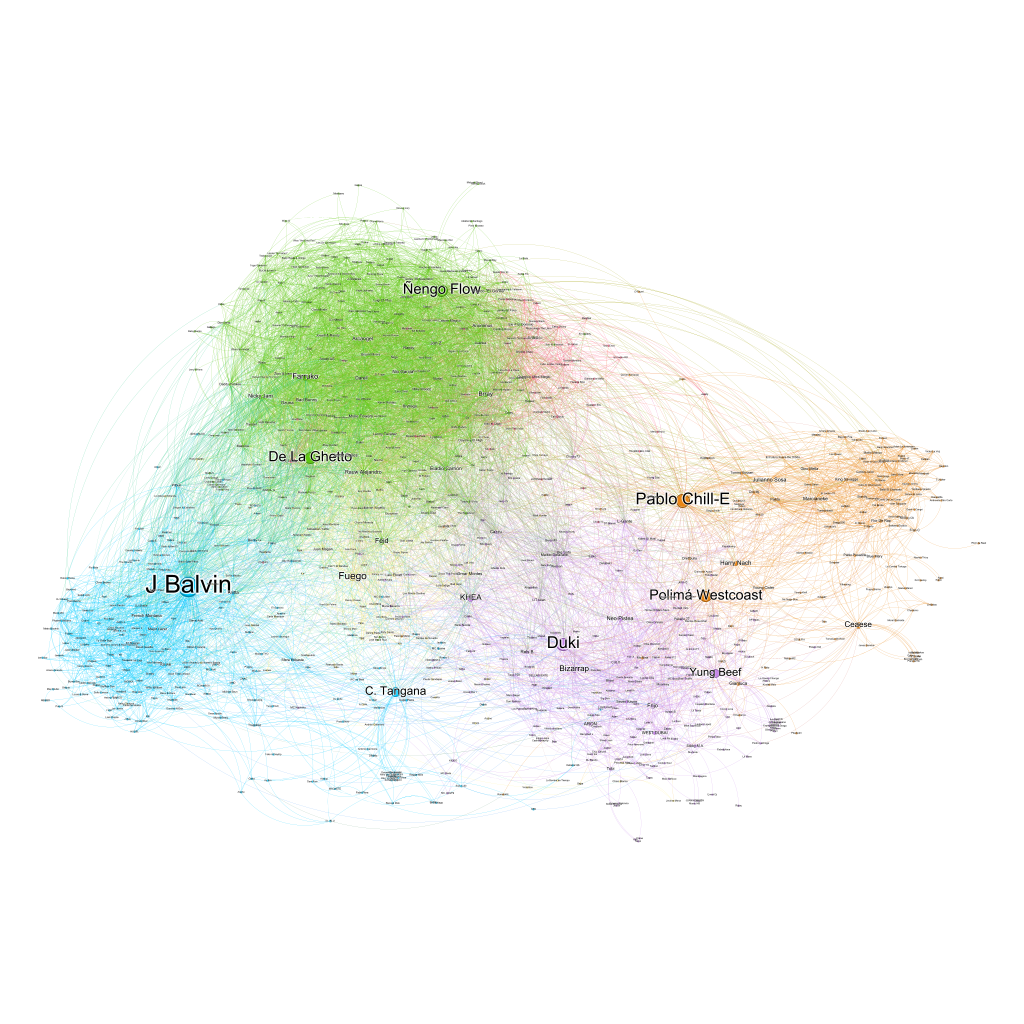
\includegraphics[width=0.61\textwidth]{PolimaWestcolModularity.png}
%    \caption{Social Network de Polimá Westcoast con comunidades detectadas por modularidad y tamaño de nodo según Betweenness}
%    \label{fig:PolimaModularity2.6}
%\end{figure}
 


\end{document}
